 \documentclass{article}

%Deutsche Sprachunterstützung
\usepackage[utf8]{inputenc}
\usepackage[ngerman]{babel}
\usepackage{marvosym}
\DeclareUnicodeCharacter{20AC}{\EUR}

%Für das Einbinden von Bildern
%\usepackage{graphicx}

%Tabellen
\usepackage{array}

%Tabellen automatisch schoener
\usepackage{booktabs}

%Caption
\usepackage{caption}
\usepackage{subcaption}

%Formeln
\usepackage{mathtools}
\usepackage{amsmath}
\usepackage{amssymb}
\usepackage{amstext}
\usepackage{dsfont}

%\usepackage{mnsymbol}

%Vectorpfeile schöner
\usepackage{esvect}

%Formatierung
\usepackage[T1]{fontenc}
\usepackage{lmodern}
\usepackage{microtype}
%\usepackage[german=guillemets]{csquotes}

%Formatierungsanweisungen
\newcommand{\wichtig}[1]{\underline{\large{#1}}}
\newcommand{\aref}[1]{(s.Abb. \ref{#1})}
\newcommand{\R}{\mathbb{R}}
\newcommand{\K}{\mathbb{K}}
\newcommand{\C}{\mathbb{C}}
\begin{document}
\section{Aufgabe 2}
\subsection{Tiefpass 1. Ordnung}
Schaltplan des Filters: \\
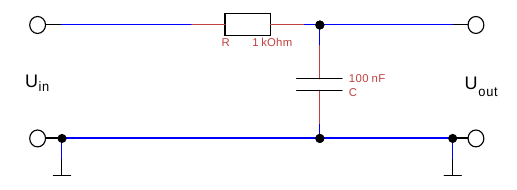
\includegraphics[width=\textwidth]{../daten/Messdaten/plots/schalt_tief}
Bode-Diagramm:\\
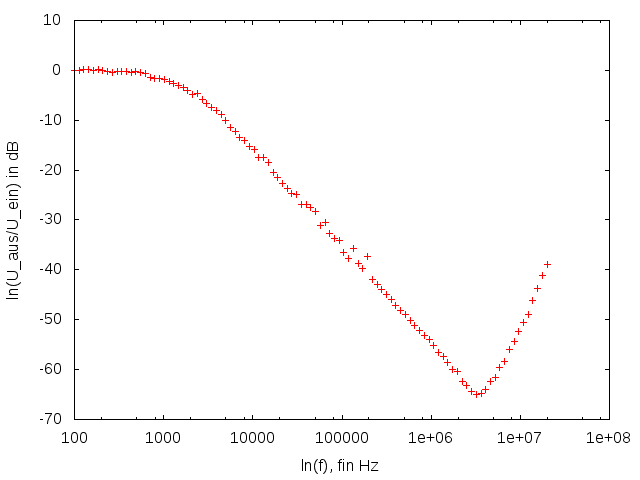
\includegraphics[width=\textwidth]{../daten/Messdaten/plots/Aufgabe2Bodediagramm_tief_gain}

Die "-3 dB-Frequenz" ist die Frequenz, bei der die ausgehende Spannung der Schaltung auf $\frac{U_{ein}}{\sqrt{2}}$ abgefallen ist. Diese Messung liefert $f_g = 1466.312710 Hz$.\\ \\
Amplitude eines 

\subsection{Hochpass 1. Ordnung}
Schaltplan des Filters:\\

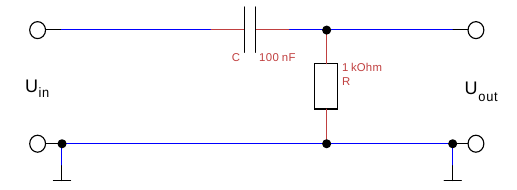
\includegraphics[width=\textwidth]{../daten/Messdaten/plots/schalt_hoch}
Bode-Diagramm:\\
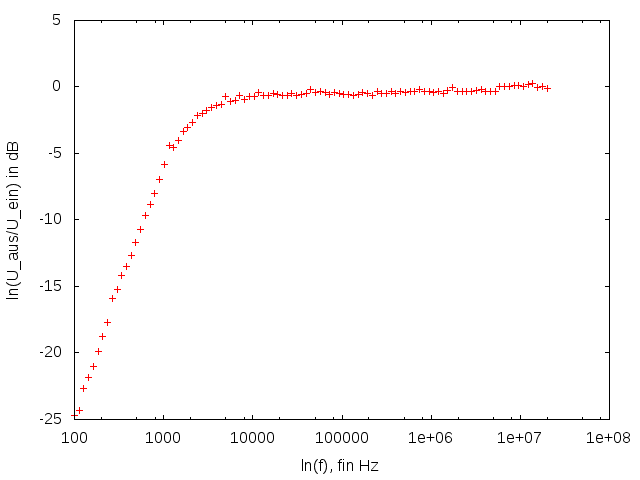
\includegraphics[width=\textwidth]{../daten/Messdaten/plots/Aufgabe2Bodediagramm_hochpass_gain}

$f_g \approx  1871.747229 Hz$

\subsection{AC-Modus des Oszilloskops}
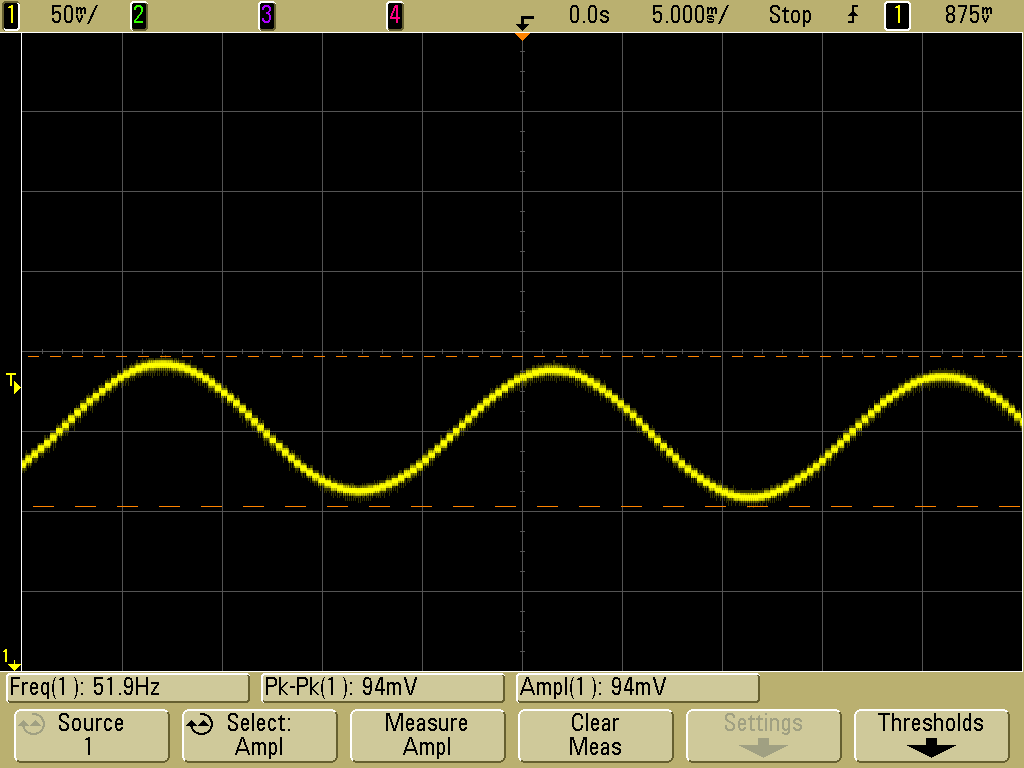
\includegraphics[width=\textwidth]{../daten/scope_16}
Signal trug zusätzlich zur Sinus-Schwingung noch eine Dreiecksspannung mit sehr niedriger Frequenz (der Verlauf deutet sich hier leicht an, da die Sinus-Welle leicht geneigt ist \\
Signal hat sich auf der Anzeige immer wieder leicht verschoben, es gab aber keine großen Probleme, es zu analysieren\\
$f_{sin} = 51.9 Hz$\\
$U_0 = 94 mV$

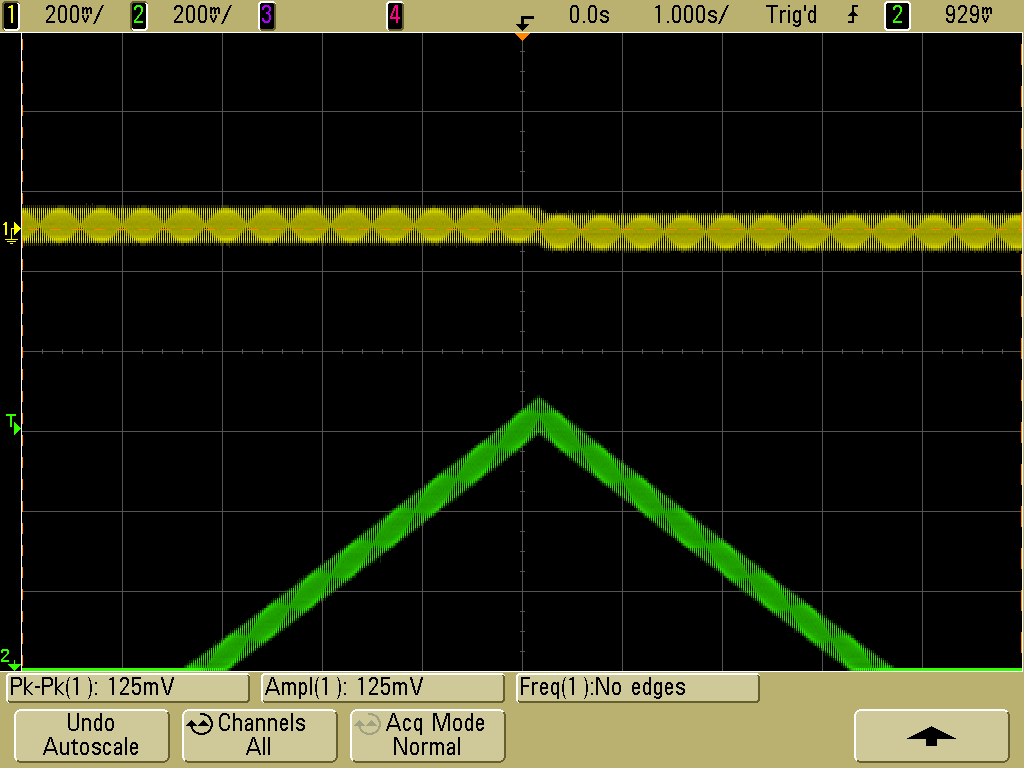
\includegraphics[width=\textwidth]{../daten/scope_21}
Vergleich zwischen Signal durch Hochpassfilter (gelb) und direkt in Oszilloskop (grün). Der Hochpass filtert die Dreiecksspannung aus dem Signal.

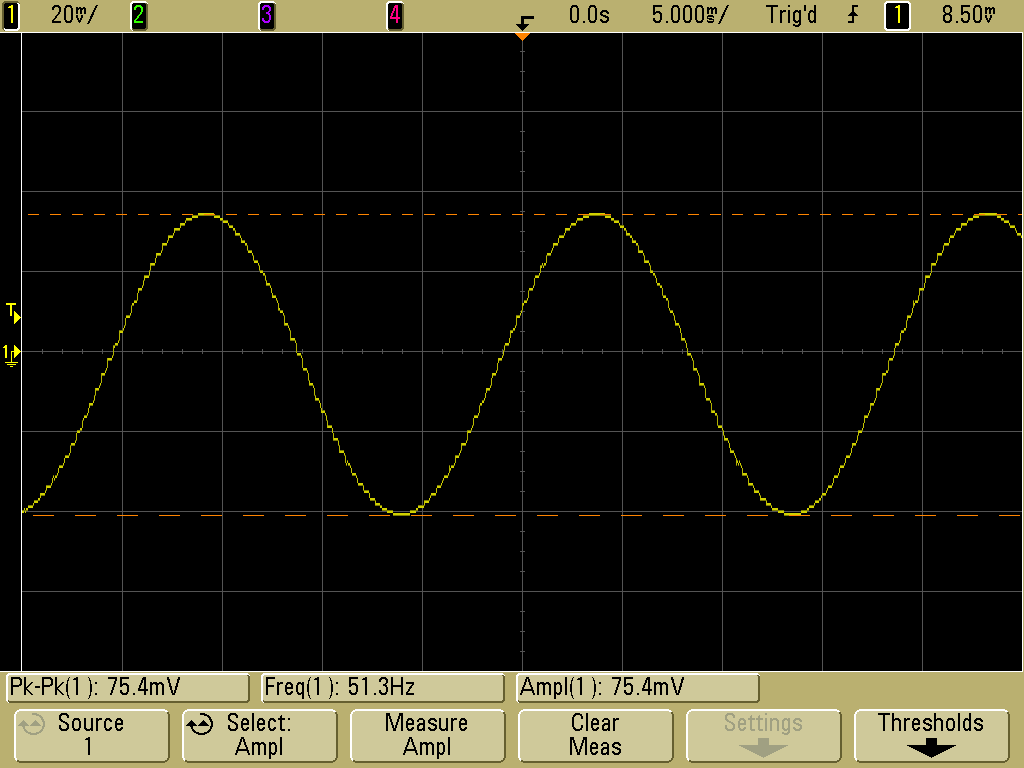
\includegraphics[width=\textwidth]{../daten/scope_22}
Mit dem AC-Modus aufgenommenes Signal\\
AC-Modus schaltet einen Hochpass-Filter zwischen Signal und Oszilloskop, der tieffrequente Schwingingen aus dem Signal entfernt
\end{document}